\part En la figura \ref{fig:triang_sem03}, el triángulo {\color{cielogris}XYZ} es semejante al triángulo {\color{strawberry}PQR}. ¿Cuál es el valor de $k$?


\begin{minipage}[t]{0.5\linewidth}
    \begin{solutionbox}{7cm}
        Los triángulos semejantes tienen lados proporcionales.

        $\Rightarrow$ podemos establecer proporciones equivalentes y resolver para $k$.

        $\therefore$
        \[
            \dfrac{k}{10.5} =\dfrac{5.5}{16.5} \]    y  \[k =3.5\]
    \end{solutionbox}
\end{minipage}
\begin{minipage}[t]{0.5\linewidth}
    \begin{figure}[H]
        \raggedright
        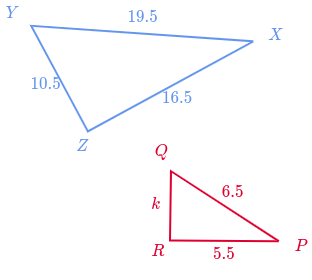
\includegraphics[width =0.8\linewidth ]{Images/triang_sem03}
        \caption{}
        \label{fig:triang_sem03}
    \end{figure}
\end{minipage}
